\documentclass{informeutn}

% --- Configuración de la Carátula ---
\titulo{Trabajo Práctico de Laboratorio Nro. 1}
\subtitulo{Error e Incertidumbre en la medición de tensión, corriente y resistencia}
\materia{Medidas Electrónicas I}
\comision{4R1} 
\autores{
    Apellido1, Nombre1 \\
    Apellido2, Nombre2 \\
    Apellido3, Nombre3 \\
    Apellido4, Nombre4
}
\fecha{\today}

\begin{document}

\maketitle

\chapter{Integrantes y Asignación de Roles}
De acuerdo a las normativas de la cátedra, los roles irán rotando a lo largo del año.
\begin{table}[H]
    \centering
    \resizebox{\textwidth}{!}{
    \begin{tabular}{|l|c|c|c|c|}
        \hline
        \textbf{Apellido y Nombres} & \textbf{Coordinador (ECG)} & \textbf{Operador 1} & \textbf{Operador 2} & \textbf{Documentación (ED)} \\ \hline
        [Nombre Estudiante 1] & X &   &   &   \\ \hline
        [Nombre Estudiante 2] &   & X &   &   \\ \hline
        [Nombre Estudiante 3] &   &   & X &   \\ \hline
        [Nombre Estudiante 4] &   &   &   & X \\ \hline
    \end{tabular}}
    \caption{Tabla de asignación de roles del grupo.}
\end{table}

\begin{itemize}
    \item \textbf{Fecha de presentación estipulada:} \dots / \dots / 2026
    \item \textbf{Fecha de coloquio grupal:} \dots / \dots / 2026
\end{itemize}

\chapter{Introducción y Objetivos}

\section{Objetivos}
\begin{itemize}
    \item Trazar la curva de contrastación de un instrumento a los fines de eliminar el error sistemático del mismo.
    \item Verificar el índice de Clase del instrumento contrastado.
    \item Determinar el valor de la resistencia en situaciones específicas (bajos valores y puestas a tierra).
    \item Dar el resultado de las mediciones acompañadas del grado de incertidumbre.
\end{itemize}

\section{Introducción Teórica}
Todo instrumento de medición presenta discrepancias entre su escala y el verdadero valor de la magnitud, debidas a tolerancias de fabricación y alinealidades. En la industria, se elaboran especificaciones estadísticas (Clase o Exactitud) para acotar este margen. Mediante la \textbf{contrastación} contra un instrumento patrón de mayor jerarquía, es posible aislar y eliminar el \textit{error sistemático}, construyendo una \textit{curva de corrección}. En este trabajo, el patrón deberá ser al menos cinco veces mejor que el instrumento bajo prueba.

Además, se estudian métodos especiales para medir \textbf{resistencias de pequeño valor}, donde el uso de un óhmetro convencional falla debido a que las \textit{resistencias de contacto} y de las puntas de prueba se suman al mensurando. El \textbf{método de 4 terminales} soluciona esto inyectando una corriente constante e independizando el circuito de medición de tensión. 

\chapter{Materiales e Instrumental}
\begin{itemize}
    \item \textbf{Multímetro Digital (Patrón):} Pro'sKit MT-1210. Exactitud: $\pm (1\% \text{ lect.} + 2 \text{ dig.})$ (hasta $200 \V$).
    \item \textbf{Multímetro Analógico (A contrastar):} Electrónico UNIVO. Exactitud declarada: $\pm 2,5 \percent$ del Fondo de Escala.
    \item \textbf{Fuente de alimentación:} Regulable de $0$ a $30 \V$.
    \item \textbf{Circuito generador de corriente constante:} Módulo basado en el regulador monolítico LM317.
    \item \textbf{Probeta a ensayar:} Tramo de cable arrollado de forma no inductiva (plegado por la mitad y luego arrollado).
    \item \textbf{Telurímetro:} UNI-T Modelo UT522.
\end{itemize}

\chapter{Desarrollo Experimental}

\section{Experimento 1: Contrastación de Voltímetro Analógico}
Se montó un esquema en paralelo entre la fuente, el multímetro analógico UNIVO y el patrón digital Pro'sKit MT-1210. 

Se procedió a variar la tensión de la fuente, alineando la aguja del UNIVO exactamente sobre las divisiones de la escala ($V_L$), y tomando la lectura del patrón digital ($V_P$). Se efectuó una pasada ascendente y una descendente para contemplar histéresis y rozamiento mecánico del galvanómetro.

\begin{table}[H]
    \centering
    \resizebox{\textwidth}{!}{
    \begin{tabular}{|c|c|c|c|c|c|c|c|c|c|c|}
        \hline
        $V_L$ [$\V$] & 1 & 2 & 3 & 4 & 5 & 6 & 7 & 8 & 9 & 10 \\ \hline
        $V_P$ (hacia arriba) & 1,01 & 2,14 & 3,20 & 4,25 & 5,32 & 6,39 & 7,46 & 8,52 & 9,59 & 10,60 \\ \hline
        $V_P$ (hacia abajo) & 0,99 & 2,11 & 3,17 & 4,23 & 5,31 & 6,38 & 7,45 & 8,51 & 9,57 & 10,60 \\ \hline
        $\Delta V$ (mayor valor) & 0,01 & 0,14 & 0,20 & 0,25 & 0,32 & 0,39 & 0,46 & 0,52 & 0,59 & 0,60 \\ \hline
    \end{tabular}}
    \caption{Valores obtenidos de la contrastación. $V_L$: indicado, $V_P$: patrón, $\Delta V$: Error absoluto.}
\end{table}

\subsection{Curva de Contrastación}
\begin{figure}[H]
    \centering
    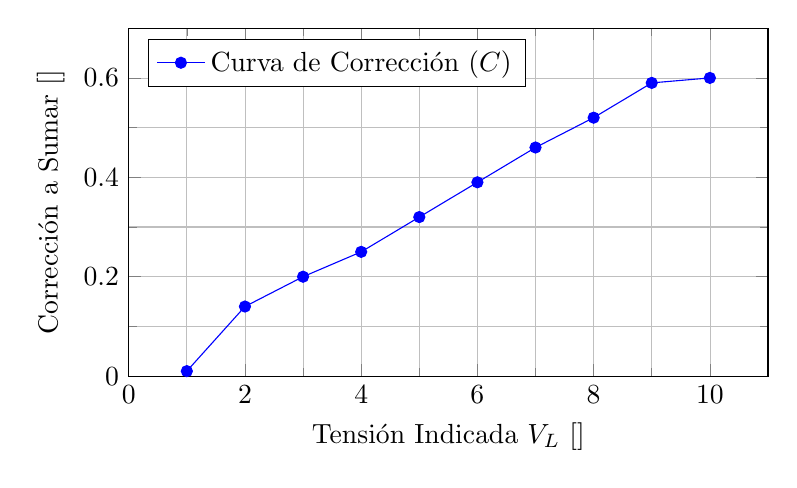
\begin{tikzpicture}
        \begin{axis}[
            width=0.8\textwidth,
            height=6cm,
            xlabel={Tensión Indicada $V_L$ [$\V$]},
            ylabel={Corrección a Sumar [$\V$]},
            xmin=0, xmax=11,
            ymin=0, ymax=0.7,
            grid=both,
            minor tick num=1,
            major grid style={line width=.2pt,draw=gray!50},
            legend pos=north west
        ]
        \addplot[color=blue, mark=*] coordinates {
            (1, 0.01)
            (2, 0.14)
            (3, 0.20)
            (4, 0.25)
            (5, 0.32)
            (6, 0.39)
            (7, 0.46)
            (8, 0.52)
            (9, 0.59)
            (10, 0.60)
        };
        \legend{Curva de Corrección ($C$)}
        \end{axis}
    \end{tikzpicture}
    \caption{Curva de contrastación: Valores a sumar al instrumento bajo prueba en función de su indicación.}
\end{figure}

\vspace{0.5cm}
\begin{table}[H]
    \centering
    \begin{tabular}{|p{4cm}|p{4cm}|c|c|}
        \hline
        \textbf{Inst. Contrastado} & \textbf{Patrón} & \textbf{Fecha y Hora} & \textbf{Operador} \\ \hline
        Marca: UNIVO \newline Nro: S/D & Marca: Pro'sKit \newline Nro: S/D & 09/04/2026 \newline 17:48 hs & Franco \newline Palombo \\ \hline
        \multicolumn{4}{|l|}{\textbf{Temperatura Ambiente:} 23 $\Celsius$} \\ \hline
    \end{tabular}
    \caption{Datos de trazabilidad de la contrastación.}
\end{table}

\subsection{Cálculo del Índice de Clase}
Del cuadro de datos, se identifica el Error Absoluto Máximo ($\Delta V = 0,60 \ \text{V}$ en $V_L = 10 \ \text{V}$) y se calcula el índice de clase:
\begin{equation}
    Clase = \frac{0,60}{10} \cdot 100 = 6 \percent
\end{equation}
\textit{(Redondear hacia arriba el resultado). Comprobación: El fabricante del UNIVO declara una Clase de $2,5$. ¿Guarda coherencia el valor obtenido?} \textbf{El valor obtenido no guarda coherencia con lo declarado por el fabricante. El instrumento presenta un índice de clase experimental del $6\%$, lo que significa que se encuentra fuera de especificación y requeriría una recalibración o reparación, ya que su error supera ampliamente el límite de $2,5\%$ del fondo de escala establecido para su correcto funcionamiento.}

\section{Experimento 2: Medición de Resistencia por 4 Terminales}
Se ajustó el generador de corriente (LM317) para entregar una corriente de prueba constante. La probeta consiste en un arrollamiento no inductivo de cable (longitud $12\text{m} \pm 12\text{cm}$).

\begin{table}[H]
    \centering
    \begin{tabular}{|c|c|c|}
        \hline
        $V$ [$\mV$] & $I$ [$\mA$] & $R = V/I$ [$\ohm$] \\ \hline
        56,8 & 100,0 & 0,568 \\ \hline
    \end{tabular}
    \caption{Medición directa de tensión y corriente en la probeta.}
\end{table}

\begin{figure}[H]
    \centering
    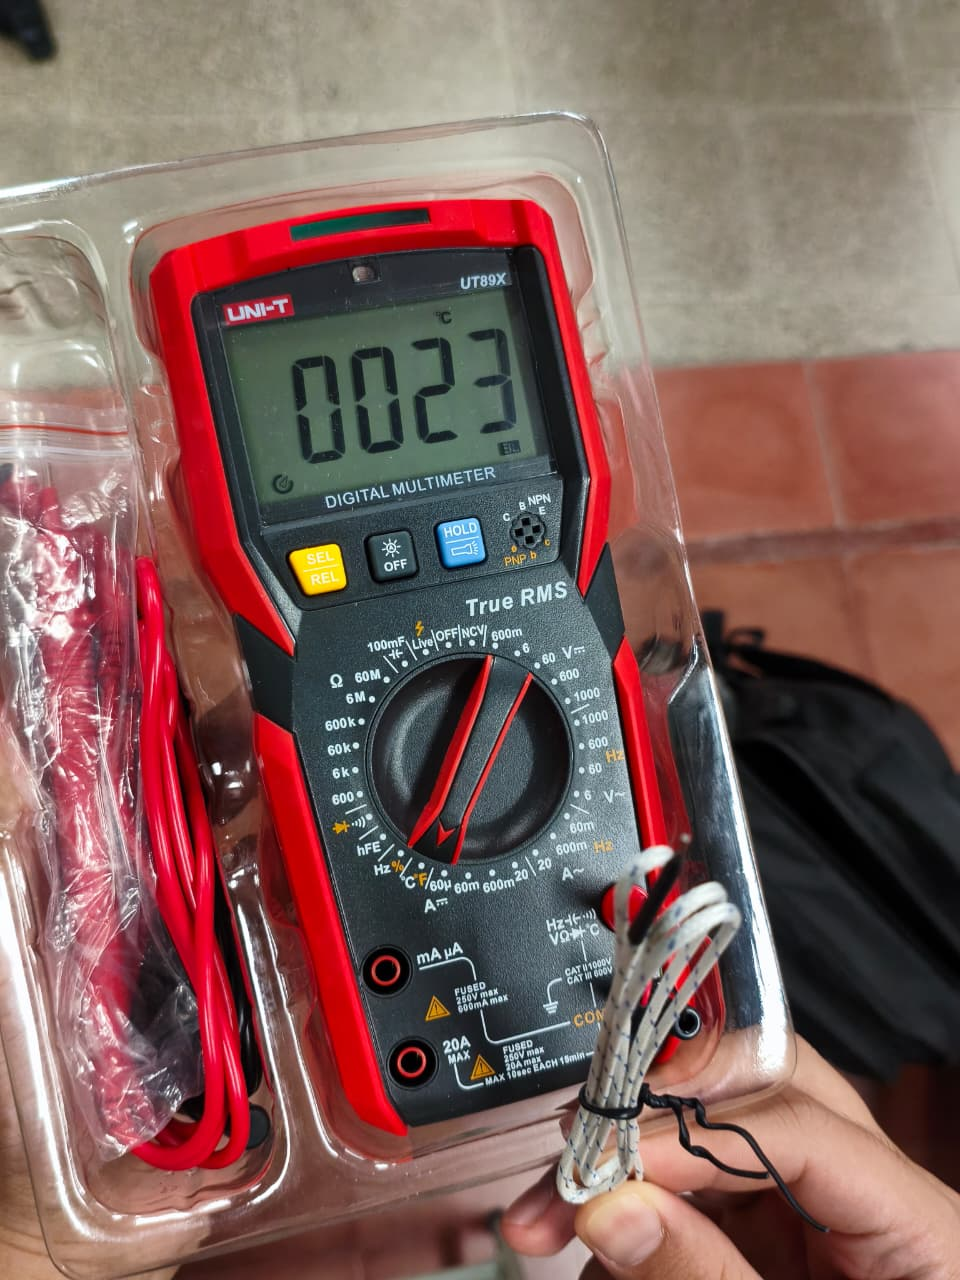
\includegraphics[width=0.7\textwidth]{foto_montaje_lm317.jpeg}
    \caption{Montaje del experimento de 4 terminales, inyectando $100\mA$ y midiendo la caída de tensión en milivoltios.}
\end{figure}

\subsection{Cálculo de la Incertidumbre}
Los errores relativos parciales se suman para obtener el error relativo máximo total de la medición indirecta de $R$:
\begin{equation}
    \frac{\Delta R}{R} = \frac{\Delta V}{V} + \frac{\Delta I}{I}
\end{equation}

Las incertidumbres $\Delta V$ y $\Delta I$ se obtienen de los manuales de los instrumentos. Para el multímetro UNI-T UT33A+ (usado como milivoltímetro en rango $200\mV$), asumimos una exactitud típica de $\pm(0.5\% + 2 \text{ dig.})$. Para el Pro'sKit MT-1210 (usado como miliamperímetro en rango $200\mA$), asumimos $\pm(1.2\% + 2 \text{ dig.})$.

\begin{table}[H]
    \centering
    \begin{tabular}{|c|c|c|c|c|}
        \hline
        Magnitud & Valor Medido & Incertidumbre Abs. ($\Delta x$) & Inc. Relativa $\left(\frac{\Delta x}{X}\right)$ & Inc. Rel. Porcentual $\left(\frac{\Delta x}{X} \cdot 100\right)$ \\ \hline
        $V$ & $56,8 \mV$ & $0,484 \mV$ & $0,0085$ & $0,85\%$ \\ \hline
        $I$ & $100,0 \mA$ & $1,4 \mA$ & $0,0140$ & $1,40\%$ \\ \hline
        $R = V/I$ & $0,568 \ohm$ & $0,013 \ohm$ & $0,0225$ & $2,25\%$ \\ \hline
    \end{tabular}
    \caption{Desglose de valores de incertidumbre.}
\end{table}

\textbf{Resultado Final:} $R = (0,568 \pm 0,013) \ \ohm$

\section{Experimento 3: Resistencia de un Sistema de Puesta a Tierra}
\textbf{Fecha de la experiencia:} Jueves 27 de Marzo en el horario de clases.

Para medir la resistencia de la jabalina del "Laboratorio Central de Electrónica" (caja ubicada debajo del pizarrón), se empleó el telurímetro UNI-T UT522 con un montaje de electrodos auxiliares sobre paños húmedos en el piso del pasillo exterior, emulando una malla conductora. Se seleccionó inicialmente el rango de $4000\ohm$.

\begin{itemize}
    \item \textbf{Valor leído $R(Jabalina)$:} \dots $\ohm$
\end{itemize}

De acuerdo al manual del instrumento, las especificaciones son:
\begin{itemize}
    \item Rango $40\ohm$: $\pm(2.0\% + 20)$
    \item Rangos $400\ohm$ y $4000\ohm$: $\pm(2.0\% + 3)$
\end{itemize}

Considerando la lectura obtenida, la incertidumbre presente en la medición es:
\begin{itemize}
    \item \textbf{$R_j$ (con incertidumbre):} $\dots \pm \dots \ \ohm$
\end{itemize}

\chapter{Conclusiones y Discusión Grupal}

A partir de la experiencia de laboratorio, el grupo de trabajo expone las siguientes resoluciones:

\begin{itemize}
    \item \textbf{Sentido de las pasadas:} ¿Cuál es el sentido de efectuar una pasada hacia arriba y otra hacia abajo durante la contrastación del voltímetro? ¿Sería mejor promediar varias series de pasadas (cuatro o cinco)? ¿Supondría ventaja o mejora?
    \\ \textit{[Respuesta...]}

    \item \textbf{Taller de mantenimiento:} Averigüe si en el Taller de mantenimiento del laboratorio el instrumental es sometido a contrastaciones periódicas.
    \\ \textit{[Respuesta...]}

    \item \textbf{Instrumentos de referencia en el laboratorio:} Elabore una lista de al menos tres instrumentos que existan en el laboratorio que podrían ser usados como referencia (patrón), incluyendo su especificación de exactitud.
    \\ \textit{[Respuesta...]}

    \item \textbf{Validez de la curva:} En el instrumento UNIVO contrastado, ¿Por cuánto tiempo estima que será válida la curva obtenida? ¿Cuáles serían las causas que obligarían a efectuar un nuevo procedimiento de contrastación?
    \\ \textit{[Respuesta...]}

    \item \textbf{Métodos de 4 terminales:} ¿Qué ventajas presentan los métodos de medición con 4 terminales por sobre los métodos convencionales (óhmetro de 2 puntas)?
    \\ \textit{[Respuesta...]}

    \item \textbf{Caja de resistencias de precisión:} Realice una búsqueda sobre "caja de resistencias de precisión". Busque hojas de especificaciones e interprete las correspondientes a la incertidumbre.
    \\ \textit{[Respuesta...]}

    \item \textbf{Regulador LM317:} La fuente de corriente propuesta es simple pero efectiva. Busque la hoja de datos del Circuito integrado LM317 e investigue cómo funciona y cómo mantiene la corriente constante.
    \\ \textit{[Respuesta...]}

    \item \textbf{Propagación de incertidumbre:} La ecuación empleada asume que los errores parciales se suman (peor caso). Algunos autores sugieren que se obtiene una mejor estimación efectuando la \textit{raíz cuadrada de la suma de los cuadrados} de los errores parciales. Compare ambos enfoques.
    \\ \textit{[Respuesta...]}
\end{itemize}

\chapter{Grilla de Evaluación}

\begin{table}[H]
    \centering
    \resizebox{\textwidth}{!}{
    \begin{tabular}{|l|p{6cm}|c|c|c|c|c|}
        \hline
        ID & Criterio de Evaluación & \%Obt. ECG & \%Obt. EO1 & \%Obt. EO2 & \%Obt. ED & \%Max \\ \hline
        CEval 1 & Identifica los datos necesarios para determinar especificaciones de los instrumentos disponibles & & & & & 10\% \\ \hline
        CEval 2 & Selecciona los instrumentos que deben ser empleados como instrumento bajo prueba y patrón & & & & & 10\% \\ \hline
        CEval 8 & Identifica los elementos necesarios para realizar el trabajo requerido & & & & & 10\% \\ \hline
        CEval 6 & Búsqueda y selección de información relevante a normativa de contrastación y calibración & & & & & 5\% \\ \hline
        CEval 9 & Búsqueda y selección de información para identificar precisión y exactitud de los instrumentos & & & & & 5\% \\ \hline
        CEval 10 & Adquiere conocimientos necesarios para correcta implementación del procedimiento & & & & & 10\% \\ \hline
        CEval 5 & Trabaja en forma grupal para completar todas las tareas establecidas & & & & & 10\% \\ \hline
        CEval 4 & Documenta con información precisa el resultado de las mediciones & & & & & 10\% \\ \hline
        CEval 3 & Realiza el informe técnico con información precisa para dar a conocer resultados & & & & & 15\% \\ \hline
        CEval 7 & Expone de forma grupal inconvenientes, experiencia y conclusiones del trabajo & & & & & 15\% \\ \hline
        \multicolumn{2}{|r|}{\textbf{TOTAL}} & & & & & \textbf{100\%} \\ \hline
    \end{tabular}}
\end{table}

\end{document}
